\documentclass[varwidth=16.0cm, border=2pt]{standalone}
\usepackage{amsmath,amssymb}
\usepackage{tikz}
\usetikzlibrary{arrows.meta}
\begin{document}
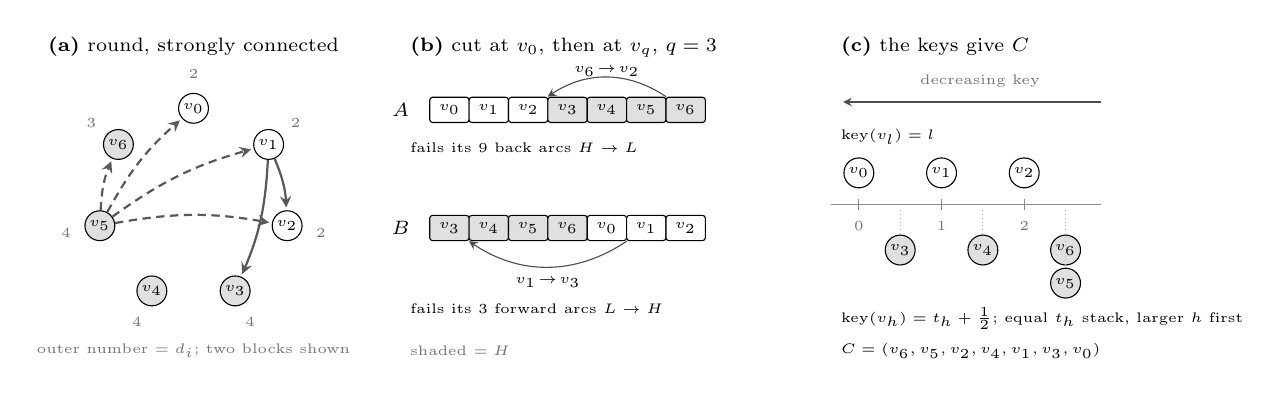
\begin{tikzpicture}[x=1cm,y=1cm]
\begin{scope}[shift={(1.90,0)}]
\node[circle,draw,inner sep=0.9pt,fill=white,font=\tiny] (w0) at (0.000,1.220) {$v_{0}$};
\node[font=\tiny,text=black!55] at (0.000,1.659) {$2$};
\node[circle,draw,inner sep=0.9pt,fill=white,font=\tiny] (w1) at (0.954,0.761) {$v_{1}$};
\node[font=\tiny,text=black!55] at (1.297,1.034) {$2$};
\node[circle,draw,inner sep=0.9pt,fill=white,font=\tiny] (w2) at (1.189,-0.271) {$v_{2}$};
\node[font=\tiny,text=black!55] at (1.618,-0.369) {$2$};
\node[circle,draw,inner sep=0.9pt,fill=black!12,font=\tiny] (w3) at (0.529,-1.099) {$v_{3}$};
\node[font=\tiny,text=black!55] at (0.720,-1.495) {$4$};
\node[circle,draw,inner sep=0.9pt,fill=black!12,font=\tiny] (w4) at (-0.529,-1.099) {$v_{4}$};
\node[font=\tiny,text=black!55] at (-0.720,-1.495) {$4$};
\node[circle,draw,inner sep=0.9pt,fill=black!12,font=\tiny] (w5) at (-1.189,-0.271) {$v_{5}$};
\node[font=\tiny,text=black!55] at (-1.618,-0.369) {$4$};
\node[circle,draw,inner sep=0.9pt,fill=black!12,font=\tiny] (w6) at (-0.954,0.761) {$v_{6}$};
\node[font=\tiny,text=black!55] at (-1.297,1.034) {$3$};
\draw[thick,->,>=stealth,black!65,shorten >=1pt] (w1) to[bend left=10] (w2);
\draw[thick,->,>=stealth,black!65,shorten >=1pt] (w1) to[bend left=10] (w3);
\draw[thick,densely dashed,->,>=stealth,black!65,shorten >=1pt] (w5) to[bend left=10] (w6);
\draw[thick,densely dashed,->,>=stealth,black!65,shorten >=1pt] (w5) to[bend left=10] (w0);
\draw[thick,densely dashed,->,>=stealth,black!65,shorten >=1pt] (w5) to[bend left=10] (w1);
\draw[thick,densely dashed,->,>=stealth,black!65,shorten >=1pt] (w5) to[bend left=10] (w2);
\node[font=\scriptsize] at (0,2.00) {\textbf{(a)} round, strongly connected};
\node[font=\tiny,text=black!55] at (0,-1.86) {outer number $=d_i$; two blocks shown};
\end{scope}
\begin{scope}[shift={(5.15,0)}]
\node[font=\scriptsize] at (-0.62,1.20) {$A$};
\node[draw,rounded corners=1pt,minimum width=0.50cm,minimum height=0.32cm,inner sep=0pt,fill=white,font=\tiny] (A0) at (0.000,1.20) {$v_{0}$};
\node[draw,rounded corners=1pt,minimum width=0.50cm,minimum height=0.32cm,inner sep=0pt,fill=white,font=\tiny] (A1) at (0.500,1.20) {$v_{1}$};
\node[draw,rounded corners=1pt,minimum width=0.50cm,minimum height=0.32cm,inner sep=0pt,fill=white,font=\tiny] (A2) at (1.000,1.20) {$v_{2}$};
\node[draw,rounded corners=1pt,minimum width=0.50cm,minimum height=0.32cm,inner sep=0pt,fill=black!12,font=\tiny] (A3) at (1.500,1.20) {$v_{3}$};
\node[draw,rounded corners=1pt,minimum width=0.50cm,minimum height=0.32cm,inner sep=0pt,fill=black!12,font=\tiny] (A4) at (2.000,1.20) {$v_{4}$};
\node[draw,rounded corners=1pt,minimum width=0.50cm,minimum height=0.32cm,inner sep=0pt,fill=black!12,font=\tiny] (A5) at (2.500,1.20) {$v_{5}$};
\node[draw,rounded corners=1pt,minimum width=0.50cm,minimum height=0.32cm,inner sep=0pt,fill=black!12,font=\tiny] (A6) at (3.000,1.20) {$v_{6}$};
\node[font=\tiny,anchor=west] at (-0.62,0.72) {fails its $9$ back arcs $H\to L$};
\node[font=\scriptsize] at (-0.62,-0.30) {$B$};
\node[draw,rounded corners=1pt,minimum width=0.50cm,minimum height=0.32cm,inner sep=0pt,fill=black!12,font=\tiny] (B0) at (0.000,-0.30) {$v_{3}$};
\node[draw,rounded corners=1pt,minimum width=0.50cm,minimum height=0.32cm,inner sep=0pt,fill=black!12,font=\tiny] (B1) at (0.500,-0.30) {$v_{4}$};
\node[draw,rounded corners=1pt,minimum width=0.50cm,minimum height=0.32cm,inner sep=0pt,fill=black!12,font=\tiny] (B2) at (1.000,-0.30) {$v_{5}$};
\node[draw,rounded corners=1pt,minimum width=0.50cm,minimum height=0.32cm,inner sep=0pt,fill=black!12,font=\tiny] (B3) at (1.500,-0.30) {$v_{6}$};
\node[draw,rounded corners=1pt,minimum width=0.50cm,minimum height=0.32cm,inner sep=0pt,fill=white,font=\tiny] (B4) at (2.000,-0.30) {$v_{0}$};
\node[draw,rounded corners=1pt,minimum width=0.50cm,minimum height=0.32cm,inner sep=0pt,fill=white,font=\tiny] (B5) at (2.500,-0.30) {$v_{1}$};
\node[draw,rounded corners=1pt,minimum width=0.50cm,minimum height=0.32cm,inner sep=0pt,fill=white,font=\tiny] (B6) at (3.000,-0.30) {$v_{2}$};
\node[font=\tiny,anchor=west] at (-0.62,-1.32) {fails its $3$ forward arcs $L\to H$};
\draw[->,>=stealth,black!70] (A6) to[bend right=34] (A2);
\node[font=\tiny,anchor=south] at (2.000,1.50) {$v_{6}\!\to\!v_{2}$};
\draw[->,>=stealth,black!70] (B5) to[bend left=34] (B0);
\node[font=\tiny,anchor=north] at (1.250,-0.80) {$v_{1}\!\to\!v_{3}$};
\node[font=\scriptsize,anchor=west] at (-0.62,2.00) {\textbf{(b)} cut at $v_0$, then at $v_{q}$, $q=3$};
\node[font=\tiny,text=black!55,anchor=west] at (-0.62,-1.86) {shaded $=H$};
\end{scope}
\begin{scope}[shift={(10.35,0)}]
\draw[black!45] (-0.35,0) -- (3.08,0);
\draw[black!45] (0.000,-0.07) -- (0.000,0.07);
\node[font=\tiny,text=black!55,anchor=north] at (0.000,-0.09) {$0$};
\node[draw,circle,inner sep=0.9pt,fill=white,font=\tiny] at (0.000,0.40) {$v_{0}$};
\draw[black!45] (1.050,-0.07) -- (1.050,0.07);
\node[font=\tiny,text=black!55,anchor=north] at (1.050,-0.09) {$1$};
\node[draw,circle,inner sep=0.9pt,fill=white,font=\tiny] at (1.050,0.40) {$v_{1}$};
\draw[black!45] (2.100,-0.07) -- (2.100,0.07);
\node[font=\tiny,text=black!55,anchor=north] at (2.100,-0.09) {$2$};
\node[draw,circle,inner sep=0.9pt,fill=white,font=\tiny] at (2.100,0.40) {$v_{2}$};
\draw[black!30,densely dotted] (2.625,-0.07) -- (2.625,-0.42);
\node[draw,circle,inner sep=0.9pt,fill=black!12,font=\tiny] at (2.625,-0.58) {$v_{6}$};
\draw[black!30,densely dotted] (2.625,-0.07) -- (2.625,-0.84);
\node[draw,circle,inner sep=0.9pt,fill=black!12,font=\tiny] at (2.625,-1.00) {$v_{5}$};
\draw[black!30,densely dotted] (1.575,-0.07) -- (1.575,-0.42);
\node[draw,circle,inner sep=0.9pt,fill=black!12,font=\tiny] at (1.575,-0.58) {$v_{4}$};
\draw[black!30,densely dotted] (0.525,-0.07) -- (0.525,-0.42);
\node[draw,circle,inner sep=0.9pt,fill=black!12,font=\tiny] at (0.525,-0.58) {$v_{3}$};
\draw[->,>=stealth,black!70] (3.08,1.30) -- (-0.20,1.30);
\node[font=\tiny,text=black!55,anchor=south] at (1.54,1.36) {decreasing key};
\node[font=\tiny,anchor=west] at (-0.35,0.86) {$\mathrm{key}(v_l)=l$};
\node[font=\tiny,anchor=west] at (-0.35,-1.45) {$\mathrm{key}(v_h)=t_h+\tfrac12$; equal $t_h$ stack, larger $h$ first};
\node[font=\scriptsize,anchor=west] at (-0.35,2.00) {\textbf{(c)} the keys give $C$};
\node[font=\tiny,anchor=west] at (-0.35,-1.86) {$C=(v_{6},v_{5},v_{2},v_{4},v_{1},v_{3},v_{0})$};
\end{scope}
\end{tikzpicture}
\end{document}
